\documentclass[addpoints]{exam}

    \makeatletter % Lagfæring fyrir nýjar útgáfur af TeXLive
    \expandafter\providecommand\expandafter*\csname ver@framed.sty\endcsname
    {2003/07/21 v0.8a Simulated by exam}
    \makeatother
    
    \usepackage[top=2cm, bottom=2cm, left=1cm, right=1cm]{geometry}
    \usepackage[utf8]{inputenc}
    \usepackage[icelandic]{babel}
    \usepackage[T1]{fontenc}
    \usepackage{helvet} \renewcommand\familydefault{\sfdefault}
    
    \usepackage[parfill]{parskip}
    \usepackage{tabularx, booktabs}
    \usepackage{multirow}
    \usepackage{multicol}
    \usepackage{graphicx, tikz}
    \usepackage{enumerate}
    \usepackage{amsmath, amsfonts, amssymb, amsthm}
    \usepackage{minted} %Minted and configuration
    \usepackage{afterpage}
    \usepackage{scrextend}
    
    \usepackage[pdftex,bookmarks=true,colorlinks=true,pdfauthor={Eirikur Ernir Thorsteinsson},linkcolor=blue,urlcolor=blue]{hyperref}
    
    \newmintedfile[cppfile]{cpp}{frame=lines, linenos=false}
    \newmintedfile[javafile]{java}{frame=lines, linenos=false}
    \newcommand{\eng}[1]{(e.\ \emph{#1})}

    \setcounter{secnumdepth}{-1} 
    \hyphenpenalty=5000
    
    \newcommand\blankpage{%
        \null
        \thispagestyle{empty}%
        \addtocounter{page}{-1}%
        }
    
    \usemintedstyle{default}
    \renewcommand{\theFancyVerbLine}{\sffamily \arabic{FancyVerbLine}}
    \author{}
    \date{}
    
    \footer{}{}{}
    
    \setcounter{secnumdepth}{-1} 
    
    \qformat{\large \textbf Spurning \thequestion \phantom{M}(\totalpoints \phantom{l}stig) \hfill}
    \renewcommand{\solutiontitle}{\noindent\textbf{Svar:}\par\noindent}
    \renewcommand{\points}{stig}
    \renewcommand{\questionshook}{\setlength{\itemsep}{0.5cm}}
    \hqword{Spurning:}
    \hpword{Stig í boði:}
    \hsword{Stig:}
    \htword{Samtals}
    
    \title{TÖL203G Tölvunarfræði 2 - upptökupróf}
    \author{}
    \date{júní 2018}
    
    \pagestyle{headandfoot}
    \firstpageheader{TÖL203G}{Tölvunarfræði 2 - Upptökupróf}{júní 2018}
    \firstpagefooter{}{Bls. \thepage\ af \numpages}{}
    \runningfooter{}{Bls. \thepage\ af \numpages}{}
    \setlength{\columnsep}{0.5cm}
    
    \changefontsizes{14pt}

\begin{document}

Fullt nafn: \vspace*{1mm} \hrule

\vspace{1cm}

\textbf{Leiðbeiningar:} Á þessu prófi eru \numquestions\ spurningar sem samtals gefa \numpoints\ stig.
Leyfileg hjálpargögn eru reiknivél og ein A4 blaðsíða af glósum.

Heftið verður skannað inn í tölvu til yfirferðar. Vinsamlegast forðist ljósa blýanta, ekki rífa eða krumpa heftið og ekki bæta við blaðsíðum eða fjarlægja.

Til að svara krossaspurningum skal nota svartöfluna hér að neðan. Merkið vandlega við einn möguleika fyrir hverja spurningu. Ekki er dregið frá fyrir röng svör.

Til að svara öðrum spurningum skal skrifa inn í svæðið sem fylgir strax á eftir hverri spurningu. Þurfi að koma viðbótarupplýsingum til skila skal skrifa það í rammana á
öftustu blaðsíðunum. Aðrir hlutar heftisins, sér í lagi bakhliðar, verða ekki lesnir.

Dæmin á þessu prófi eru misþung. Þau eru ekki sett fram í erfiðleikaröð.

\begin{center}
	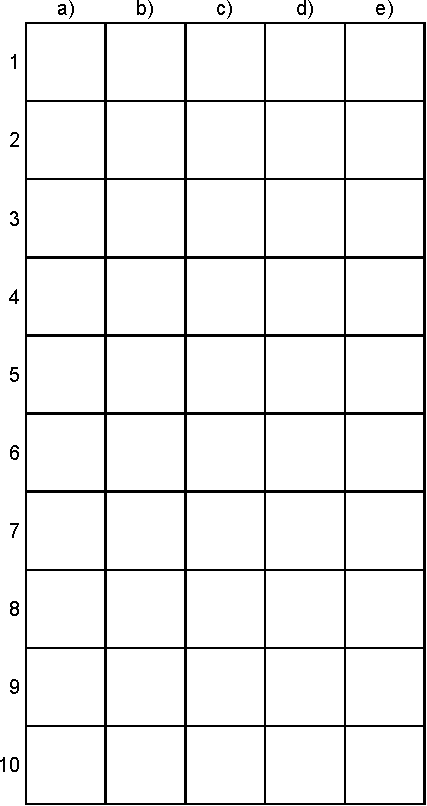
\includegraphics[width=0.4\linewidth]{Pics/svartafla}
\end{center}

\newpage

\begin{questions}

	\section{Krossaspurningar}

	\question[3]

	Gefinn er C++ forritsbútur. Hvað skrifar hann út?
	\begin{multicols}{2}

		\cppfile[firstline=3, gobble=4, lastline=8]{Code/w14/Arrayoutofbounds.cpp}

		\begin{enumerate}[a)]
			\item 0
			\item 1
			\item Forritið fer í endalausa lykkju
			\item Forritið þýðist ekki
			\item Virkni forritsins er óskilgreind % Rétt
		\end{enumerate}
	\end{multicols}

	\question[3] Þegar \texttt{new} er notað við skilgreiningu á C++ breytu verður líftími hennar\ldots

	\begin{enumerate}[a)]
		\item Frumstæður \eng{primitive}
		\item Kyrrstæður \eng{static}
		\item Kvikstæður \eng{dynamic} % Rétt
		\item Sérstæður \eng{particular}
		\item Sjálfvirkur \eng{automatic}
	\end{enumerate}

	\question[3]
	Gefið er eftirfarandi C++ fall. Hvert er vandamálið við það?

	\begin{multicols}{2}
		\begin{minted}[frame=lines]{cpp}
int* f( int a ) {
    int b = 2*a;
    return &b;
}
        \end{minted}

		\begin{enumerate}[a)]
			\item Fallið er málfræðilega rangt
			\item Fallið skilar ekki bendi á heiltölu
			\item Fallið tekur ekki frá minni fyrir \texttt{b}
			\item Fallið skilar alltaf \texttt{nullptr}
			\item Fallið skilar minnissvæði af hlaðanum % Rétt
		\end{enumerate}
	\end{multicols}

	\question[3]

	Hver eftirfarandi C++ skipana sækir minnissvæði staks númer 2 í fylkinu \texttt{c}?

	\begin{multicols}{5}
		\begin{enumerate}[a)]
			\item \texttt{*c[2]}
			\item \texttt{\&c[2]} %Rétt
			\item \texttt{?c[2]}
			\item \texttt{\#c[2]}
			\item \texttt{c[1]++}
		\end{enumerate}
	\end{multicols}

	\newpage

	\question[3]

	Hvert af eftirfarandi á við um eintengda lista?

	\begin{enumerate}[a)]
		\item Uppfletting í lista er almennt skilvirkari en í fylki
		\item Tímafrekt er að bæta staki við fremst í lista
		\item Listar geta geymt meiri upplýsingar en fylki því þeir eru geymdir í kös
		\item Auðveldara er að fjölga stökum í lista en í fylki % Rétt
		\item Listar þurfa minna minni en fylki til að geyma hvert stak
	\end{enumerate}

	\question[3]

	Sé hlaði \eng{stack} útfærður á skynsamlegan hátt með eintengdum lista, af hvaða stærðargráðu er tími innsetningar og eyðingar á $N$ staka hlaða?

	\begin{enumerate}[a)]
		\item  $1$ (fasti) innsetning og eyðing % Rétt
		\item  $\log N$ innsetning og eyðing
		\item  $1$ innsetning, $N$ eyðing
		\item  $N$ innsetning, $1$ eyðing
		\item  $N$ innsetning og eyðing
	\end{enumerate}

	\question[3]
	Af hvaða stærðargráðu er meðalkeyrslutími innsetningarröðunar á $N$ staka fylki?

	\begin{multicols}{5}
		\begin{enumerate}[a)]
			\item $1$ (fasti)
			\item $\log N$
			\item $N$
			\item $N\log N$
			\item $N^2$ % Rétt
		\end{enumerate}
	\end{multicols}

	\question[3]
	$N$ lyklar eru settir í slembinni röð inn í nafnatöflu sem útfærð er með rauðsvörtu tré. Af hvaða stærðargráðu verður keyrslutími einnar uppflettingar í nafnatöflunni?

	\begin{multicols}{5}
		\begin{enumerate}[a)]
			\item $1$ (fasti)
			\item $\log N$ % Rétt
			\item $N$
			\item $N\log N$
			\item $N^2$
		\end{enumerate}
	\end{multicols}

	\question[3]
	$N$ lyklar eru settir í slembinni röð inn í forgangsbiðröð sem útfærð er með röðuðu fylki. Af hvaða stærðargráðu er heildarinnsetningartíminn?

	\begin{multicols}{5}
		\begin{enumerate}[a)]
			\item $1$ (fasti)
			\item $\log N$
			\item $N$
			\item $N\log N$
			\item $N^2$ % Rétt
		\end{enumerate}
	\end{multicols}

	\newpage

	\question[3]

	Hvert eftirfarandi reiknirita má nota til að finna léttasta spanntré í vegnu neti?

	\begin{enumerate}[a)]
		\item Dýptarleit
		\item Breiddarleit
		\item Reiknirit Prims % Rétt
		\item Reiknirit Dijkstras
		\item Reiknirit Sedgewicks
	\end{enumerate}

	\section{Skrifleg verkefni}

	\question[5]

	Í útfærslu Sedgewicks og Wayne á reikniriti Dijkstras er endurtekið ``slakað á'' örvaleggjum (með aðferðinni \texttt{relax}). Útskýrið stuttlega hvað felst í því að slaka á örvalegg frá hnúti \texttt{v} til hnúts \texttt{w}.

	\makeemptybox{\stretch{1}}

	\newpage

	\question[5]

	Lýsið því hvernig árekstrar eru útkljáðir í “linear probing” hakkatöflu.

	\makeemptybox{\stretch{1}}

	\question[5]

	Nefnið einn kost sem quicksort hefur umfram innsetningarröðun og einn kost sem innsetningarröðun hefur umfram quicksort.

	\makeemptybox{\stretch{1}}

	\newpage

	\question[5]

	Teiknið einfalt tvíleitartré sem liggur að baki nafnatöflu. Sýnið ástandið eftir að að lyklarnir T O L V U N A R F R A E D I eru settir inn í töfluna í röð, væri hún tóm í upphafi. Látið gildin vera númer lykilsins (í innsetningarröð, fyrsta talan 0).

	\makeemptybox{\stretch{1}}

	\newpage

	\section{Forritunarspurningar}

	\question[10] Skrifið Java-aðferðina \texttt{swap} sem tekur inn tvo hlaða og skiptir á stökum þeirra, þannig að \texttt{s1} innihaldi öll stök sem upphaflega voru í \texttt{s2} og öfugt. Röð stakanna á að vera sú sama og í upphafi.

	Haus aðferðar: \texttt{void swap(Stack<Item> s1, Stack<Item> s2)}

	\makeemptybox{\stretch{1}}

	\newpage

	\question

	Í viðauka er gefinn hluti af útfærslu á biðröð í C++.

	\begin{parts}

		\part[5] Skrifið aðferðina \texttt{enqueue}, sem bætir nýju staki við biðröðina. Aðferðin skal taka fastan tíma í keyrslu.

		\makeemptybox{\stretch{1}}

		\part[5] Klárið aðferðina \texttt{dequeue}, sem fjarlægir það stak sem lengst hefur verið í biðröðinni. Aðferðin skal taka fastan tíma í keyrslu.

		\makeemptybox{\stretch{1}}

	\end{parts}

	\newpage

	\question[10]

	Útfærið quicksort í Java. Gefin er aðferðin \texttt{partition} sem hefur eftirfarandi haus:
	\begin{center}
		\texttt{int partition(Comparable[] a, int lo, int hi)}
	\end{center}
	Hún endurraðar stökunum \texttt{a[lo...hi]} svo að \texttt{a[lo...j-1] <= a[j] <= a[j+1...hi]} og skilar vísinum \texttt{j}.

	Haus röðunaraðferðar: \texttt{void sort(Comparable[] a)}.

	\makeemptybox{\stretch{1}}

	\newpage

	\question[10]

	Skrifið aðferð í Java sem tekur inn fylki af \texttt{Comparable} stökum sem við túlkum sem hrúgu, ásamt heiltölu \texttt{k}. Aðferðin skal skila sönnu ef hluttréð sem hefst í \texttt{k} uppfyllir hrúguskilyrði, annars ósönnu.

	Hrúgan er max-hrúga og gerum ráð fyrir að stak númer 0 í fylkinu sé tómt.

	Haus aðferðar: \texttt{boolean isMaxHeap(Comparable[] a, int k)}.

	\makeemptybox{\stretch{1}}

	\newpage

	\question[10]

	Stefnd net án örvarása hafa þann eiginleika að fyrir þau má finna röðun \eng{topological ordering} svo að allir leggir netsins vísi í sömu átt þegar netið er teiknað. Sjá mynd í viðauka. Skrifið Java-aðferðina \texttt{ordering} sem tekur inn stefnt net (\texttt{Digraph}) ásamt númeri á upphafshnúti og skilar slíkri röðun sem runu af hnútanúmerum (t.d. fylki eða \texttt{Iterable} hlut). Gera má ráð fyrir að netið sé sannarlega rásalaust og hunsa má hnúta sem ekki eru aðgengilegir frá upphafshnútnum.

	\makeemptybox{\stretch{1}}

	\paragraph{Ábending:} Hægt er að nota aðferð sem líkist dýptarleit.


\end{questions}

\newpage

\section{Viðbótarpláss}

Eftirfarandi viðbótarpláss verður skannað inn. Sé það notað, vísið til þess í viðkomandi spurningu.

\makeemptybox{\stretch{1}}

\newpage

\makeemptybox{\stretch{1}}

\newpage

\section{Viðauki}

Eftirfarandi skil úr \emph{Algorithms, 4th edition} eru gefin:
\begin{center}

    

    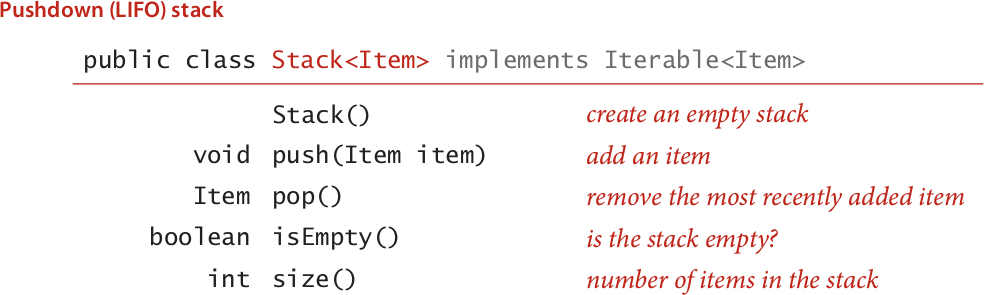
\includegraphics[width=0.6\textwidth]{Pics/API-Stack}

    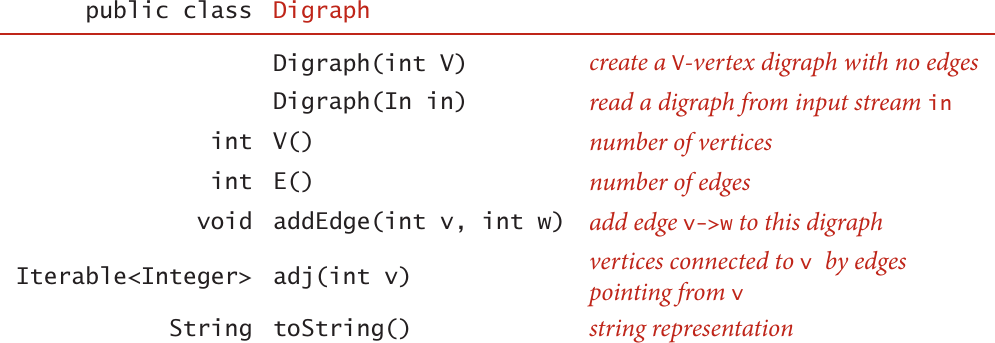
\includegraphics[width=0.7\textwidth]{Pics/API-Digraph}

    \begin{multicols}{2}
    Klasi sem táknar biðröð fyrir spurningu 16:

        \cppfile[fontsize=\scriptsize, firstline=3, lastline=37]{Code/w14/Queue.cpp}

	Til vinstri: Stefnt rásalaust net. Til hægri: Röðunin 2 0 1 4 3 á netinu.

	\usetikzlibrary{arrows}
	\begin{tikzpicture}
		\tikzset{edge/.style = {->,> = latex'}}
		\node (c1) at (2, 3) {2};
		\node (d1) at (3, 2) {0};
		\node (e1) at (3, 4) {1};
		\node (f1) at (0, 3) {4};
		\node (g1) at (0, 1) {3};

		\draw[edge] (c1) to (f1);
		\draw[edge] (c1) to (g1);
		\draw[edge] (d1) to (e1);
		\draw[edge] (e1) to (f1);
        \draw[edge] (c1) to (d1);

		\node (c2) at (6, 1) {2};
		\node (d2) at (6, 2) {0};
		\node (e2) at (6, 3) {1};
		\node (f2) at (6, 4) {4};
		\node (g2) at (6, 5) {3};

		\draw[edge] (c2) to[bend right=70] (f2);
		\draw[edge] (c2) to[bend left=70] (g2);
		\draw[edge] (d2) to (e2);
		\draw[edge] (e2) to (f2);
        \draw[edge] (c2) to (d2);
    \end{tikzpicture}
    \end{multicols}

\end{center}
\end{document}